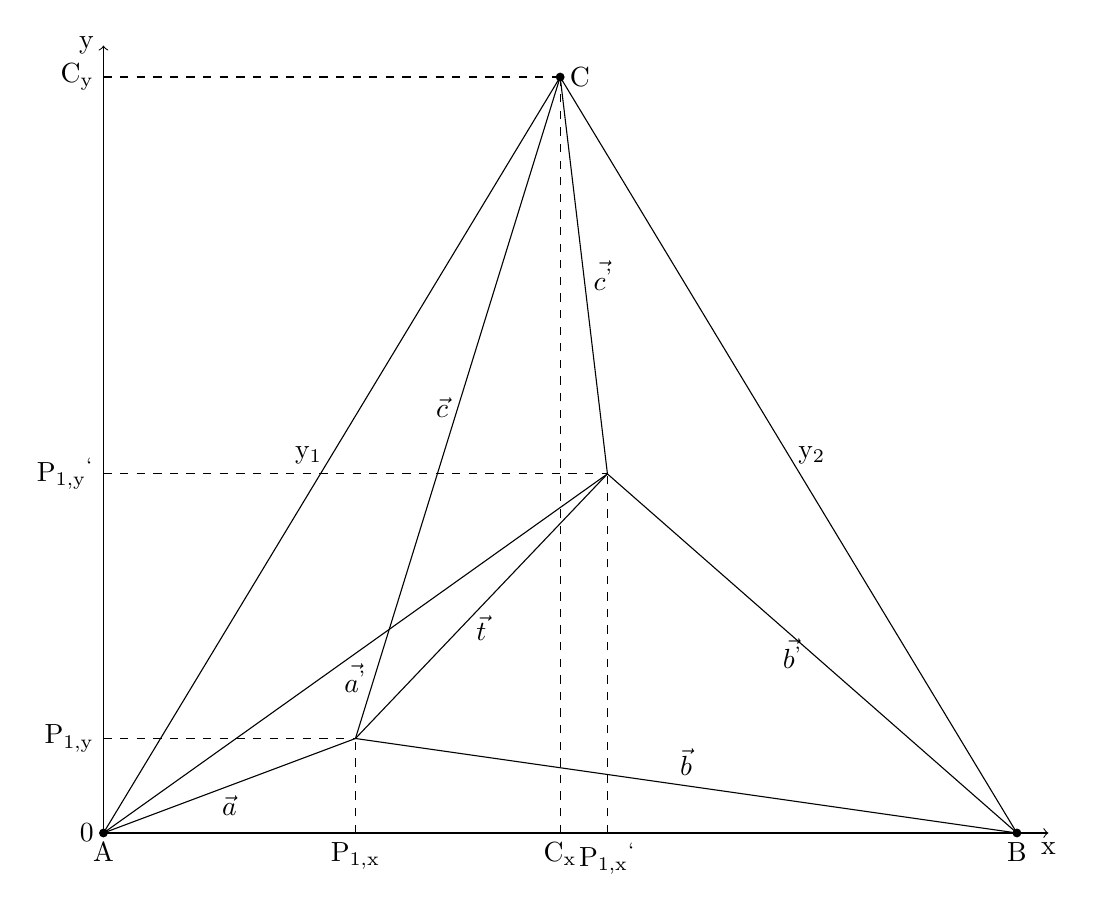
\begin{tikzpicture}[scale=0.8]
\coordinate 	[label=left:0]										(Nullpunkt) at (0,0);
\coordinate		[label=below:A] 									(A) 		at (0,0);
\coordinate		[label=below:B] 									(B) 		at (14.5,0);
\coordinate		[label=right:C] 									(C) 		at (7.25,12);

\coordinate	(P1) 		at (4,1.5) ;
\coordinate	(P1') 		at (8,5.7);

\coordinate		[label=below:x]										(X) 		at (15,0);
\coordinate		[label=left:y]										(Y) 		at (0,12.5);

\coordinate		[label=left:C\textsubscript{y}]						(YC)		at (0,12);
\coordinate		[label=below:C\textsubscript{x}]					(XC)		at (7.25,0);

\coordinate		[label=left: P\textsubscript{1,y}]					(YP1)		at (0,1.5);
\coordinate		[label=below:P\textsubscript{1,x}]					(XP1)		at (4,0);
\coordinate		[label=left: P\textsubscript{1,y}\textsuperscript{`}](YP1')		at (0,5.7);
\coordinate		[label=below:P\textsubscript{1,x}\textsuperscript{`}](XP1')		at (8,0);

\draw [->]		(Nullpunkt) -- (X)		;
\draw [->]		(Nullpunkt) -- (Y)		;
\draw 			(A) 		-- (B)		;
\draw 			(B) 		-- (C) 		node[midway,right] 	{y\textsubscript{2}};
\draw 			(C) 		-- (A) 		node[midway,left] 	{y\textsubscript{1}};
\draw 			(A) 		-- (P1) 	node[midway,below] 	{$\vec{a}$};
\draw 			(A) 		-- (P1')	node[midway,below] 	{$\vec{a\textsuperscript{'}}$};
\draw 			(B) 		-- (P1) 	node[midway,above] 	{$\vec{b}$};
\draw 			(B) 		-- (P1')	node[midway,left] 	{$\vec{b\textsuperscript{'}}$};
\draw 			(C) 		-- (P1) 	node[midway,left]  	{$\vec{c}$};
\draw 			(C) 		-- (P1')	node[midway,right]  {$\vec{c\textsuperscript{'}}$};
\draw 			(P1) 		-- (P1')	node[midway,below]  {$\vec{t}$};

\draw [dashed]  (YC) 		-- (C)		;
\draw [dashed]  (XC) 		-- (C)		;

\draw [dashed]  (YP1) 		-- (P1)		;
\draw [dashed]  (XP1) 		-- (P1)		;
\draw [dashed]  (YP1') 		-- (P1')	;
\draw [dashed]  (XP1') 		-- (P1')	;

\fill (A) circle (2pt);
\fill (B) circle (2pt);
\fill (C) circle (2pt);
\end{tikzpicture}
\caption{Darstellung der Transformation eines Punktes im Zweidimensionalen}
				